%sri
\section{Introduction}

Failures during large-scale executions of applications on extreme-scale systems
lead to loss of time and money, and are a nightmare to any application
developer. While failures could be due to application bugs, failures due
to errors not detectable by error correcting code (ECC) are on the rise.  For
example, Geist states that such failures are a common occurrence on Oak Ridge
National Laboratories leadership class machines~\cite{errors_ecc}, and
Schroeder and Gibson state that a large number of CPU and memory failures were
from parity errors after tracking a five-year log of hardware replacements for
a $765$ node high-performance computing cluster~\cite{schroeder_gibson}. We 
believe it is c

To address
these failures, we believe 

that programming models targetting extreme-scale systems should provide the ability to recover from such failures. Among these programming models,
Legion stands out to us as an exa-scale ready programming model, and hence, in
this paper develop a ..... for legion


introduce 

With the advent of productive programming models like Legion~\cite{legion}, X10~\cite{x10}, 
PARSEC~\cite{parsec}, CHARM++~\cite{charm++}, and others, programming extreme-scale
systems is not as significant a challenge as addressing other 




what are the challenges we face with resilience in a deferred execution model,
with all the decisions taken at runtime via a mapper ? \\

what are the advantages that we derive from the same ?\\ The needle in the
resilience spectrum can be much finer than ABFT, sub-tree DAG based, snapshot
based, relocatable-finish based, strategies. Dynamic and deferred being the
key.

what are the advantages that we derive from having multiple wavefront ?\\ how
do we ensure minimal overhead ?\\

Is it really a resilience framework, or a glorified garbage collector ?\\


how is it different from x10, parsec, charm++\\
	- they also allow tasks to be marked as resilience\\
	- x10 allows finish blocks, exception semantics.\\
	- what are the exception semantics that we are providing\\


what about regent ? where do we stand there ?\\

what about local vs global recovery\\
	- can we recover from a node failure\\
	- can we recover from an exception, what are the semantics that we provide
	  here\\
	- can we recover from ECC errors, \\
	- can we fix these errors ?\\
	- can we recover from I/O errors ?\\ 
	- can we recover from non-SingleTasks, what is recovery for index space
	  tasks, must epoch tasks\\

what is the memory consistency model ? what is the state of the regions, the
tasks that are physically dependent but are not logically dependent ?\\
	

experiments: circuit, miniAero, Soleil-X, stencil, (S3D ?)\\

\begin{figure}
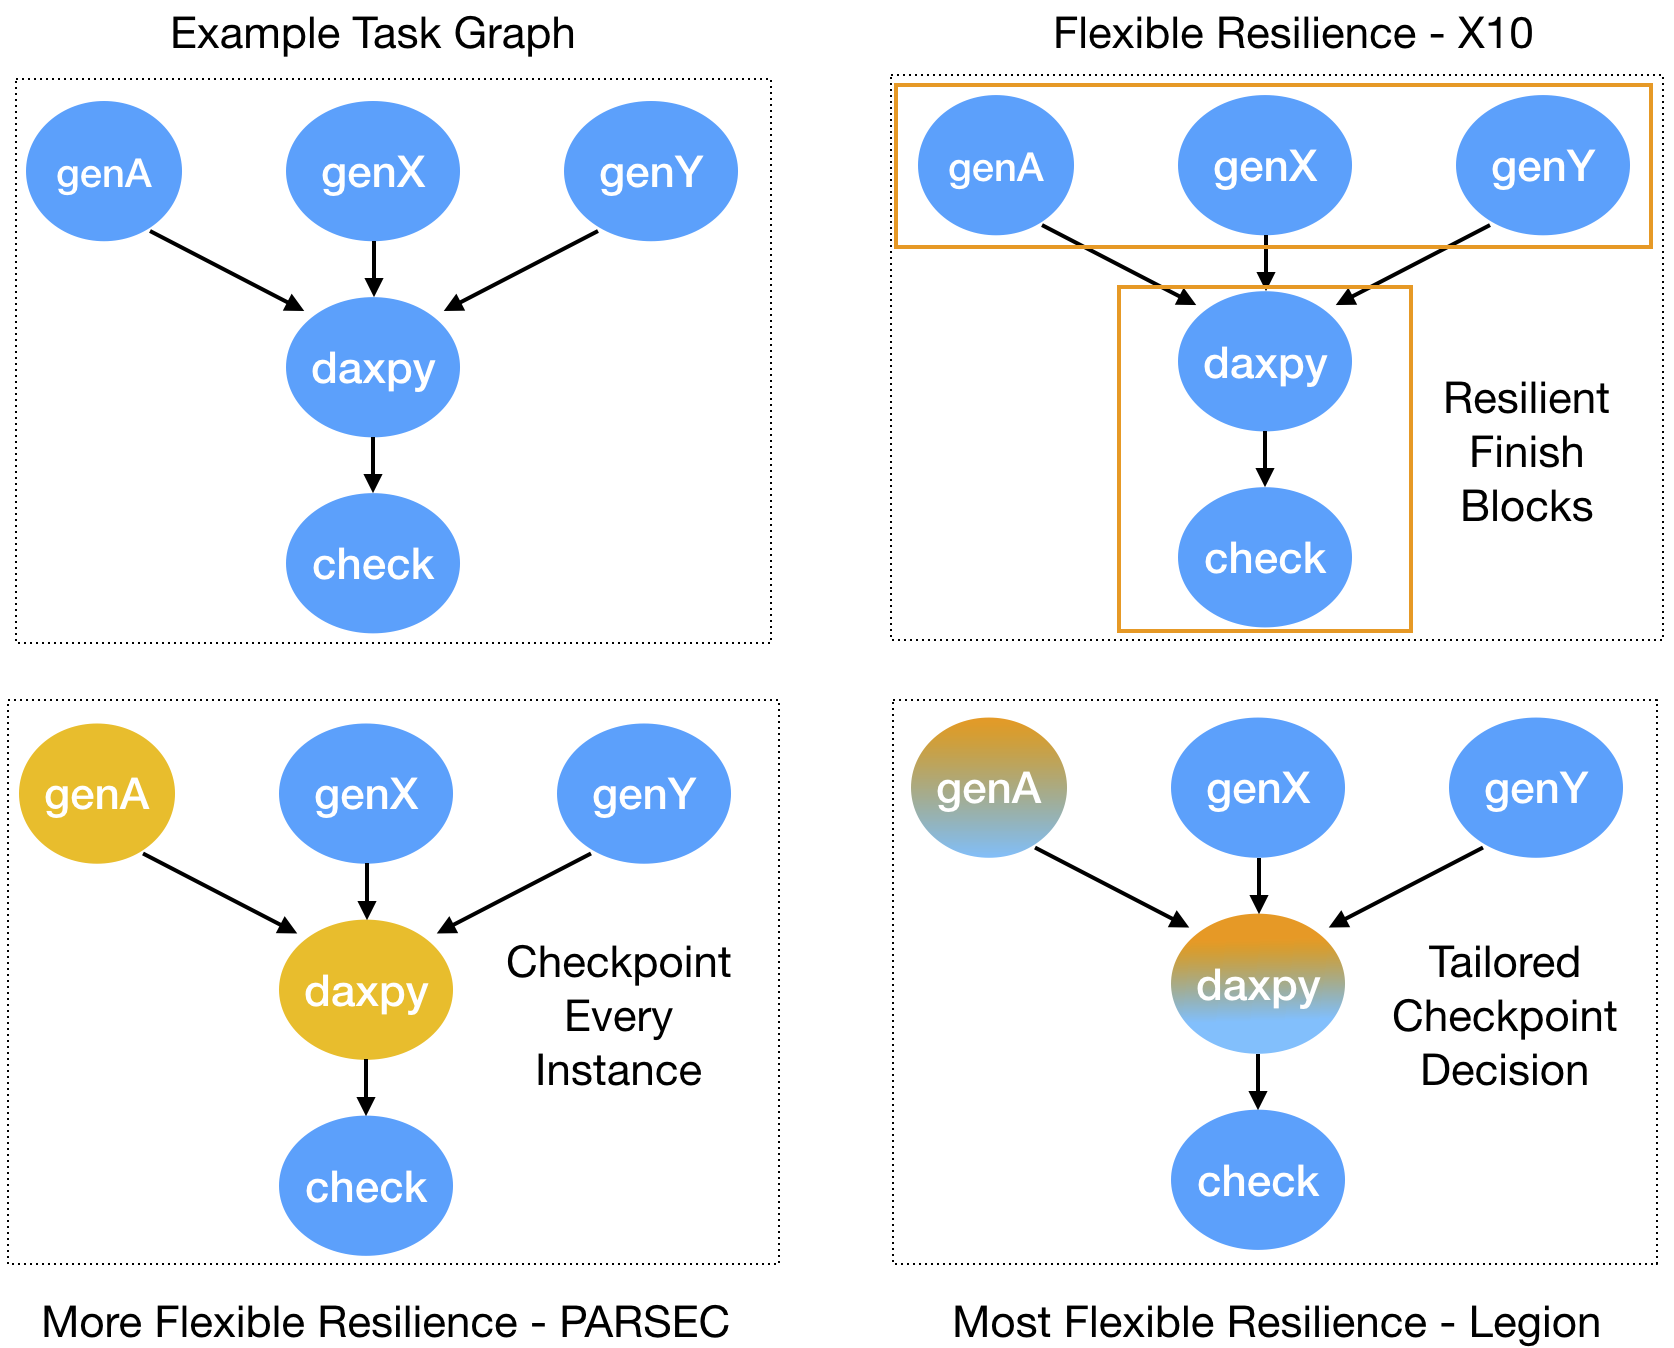
\includegraphics[width=.40\textwidth]{images/spectrum_x10_parsec_legion_policies.png}
\caption{A spectrum of resilience policies supported by different state-of-the-art parallel runtimes.}
\end{figure}

Our contributions are as follows:
\begin{itemize}
\item 
\end{itemize}


The rest of the paper is organized as follows:
